\chapter{Experimente}
\label{chap:experiments}

\section{Datens"atze}
\label{sec:datasets}

Der vorgestellte Algorithmus wird auf zwei Datensätzen evaluiert: Einerseits wird ein allgemeiner Datensatz zur Überprüfung der Ergebnisse genutzt, aber auch ein domänenspezifischer Datensatz, über den die Analyse der Marsoberfläche evaluiert wird. 

\subsection{Domänenspezifisch}

Die in Kapitel~\ref{chap:experiments} genutzten, domönenspezifischen Datensätze stammen von der Website des \textit{Planetary Data System} der NASA \cite{pds}, \bzw dem \textit{Planetary Science Archive} der ESA \cite{psa}. Die dort gehosteten Aufnahmen der jeweiligen Instumente sind größtenteils unverarbeitet und befinden sich in einem speziell für diesen Zweck erstellten Dateiformat, sodass diese erst konvertiert und anschließend so verarbeitet werden müssen, dass für diesen Zweck besser geeignete Bilddateien entstehen.
Diese Verarbeitung besteht bei den Aufnahmen der CTX aus dem Herunterladen der Metadaten der einzelnen Aufnahmen, gefolgt von der Konvertierung der Pixelfarbwerte, der Entfernung der Even/Odd Detector Stripes, und der Ausgabe in ein adäquates Bildformat. Dieses kann von dem eigentlichen Analyse-Algorithmus eingelesen und weiter verarbeitet werden. Bei den Aufnahmen der HRSC ist keine Konvertierung notwendig, diese müssen nur entsprechend konvertiert werden.

Es existieren allerdings keine segmentierten Aufnahmen der Marsoberfläche. Aus diesem Grund wird der in Unterabschnitt~\ref{ssec:crater_detection_nn} Datensatz genutzt. Da dieser allerdings nur Informationen über die Positionen der Krater auf der Marsoberfläche zur Verfügung stellt, werden die durch den hier vorgestellten Algorithmus erzeugten Segmentieren manuell in zwei Klassen eingeordnet: Krater und Nicht-Krater.

\subsection{Allgemein}

Ein oft genutzter Datensatz zu Evaluierung von Segmentierungsalgorithmen ist der Common Objects in Context-Datensatz (COCO) \cite{lin_14}. Zu diesem Datensatz existieren unterschiedliche AUfgaben \bzw Herausforderungen inkl. Ergebnissen, mit welchen man die jeweils eignen Ansätze vergleichen kann. Hier wird der sog. \textit{COCO 2017 Stuff Segmentation Task} genutzt.

\section{Evaluation}
\label{sec:evaluation}

\subsection{Domänenspezifisch}

\subsection{Allgemein}

\section{Resultate}
\label{sec:results}

\section{Vergleich}
\label{sec:comparision}

\section{Mosaik}
\label{sec:mosaic}

\iffalse
\chapter{Experimente}
\label{chap:experimente}

\section{Datens"atze}
\label{sec:datensätze}


Als allgemeiner Datensatz wird das Berkeley Segmentation Dataset \cite{bsd500} genutzt. Dieses besteht aus 500 Foto-Aufnahmen, die manuell segmentiert wurden.



\section{Evaluation}
\label{sec:Evaluation}

Zur Evaluierung und zum Vergleich der einzelnen Ansätze werden Metriken benötigt, die die verschiedenen Stärken und Schwächen der jeweiligen Lösungen zu einem Wert zusammenfassen. Hierbei ist zu beachten, dass ein Großteil der in anderen Arbeiten verwendeten Metriken wie \bspw der $F_1$-Score an dieser Stelle nicht geeignet sind, da diese voraussetzen, dass das jeweilige Bild nicht nur segmentiert, sondern diese Segmente auch eine bestimmten Klasse zugeordnet sind. Da der hier vorgestellte Ansatz nicht-zugeordnete Cluster erzeugt, weichen wir auf den Rand Index\cite{randindex} aus. Dieser ist wie folgt definiert:
% TODO Herleiten
\[R=\frac{a+b}{\binom{n}{2}}\]

Der F1-Score wird lediglich dazu genutzt, um eine berechnete Segmentierung, in der manuell die entsprechenden Label, die Krater darstellen, mit anderen Methoden zur Kratererkennung zu vergleichen. (\vgl Unterabschnitt~\ref{ssec:f1_crater})

\section{Resultate}
\label{sec:resultate}

\section{Vergleich}
\label{sec:vergleich}

Wie in Unterabschnitt~\ref{ssec:vergleich} beschreiben, wurden drei bekannte Algorithmen zur Kratererkennung  (Urbach '09 \cite{urbach_stepinski_2009}, Bandeira '10 \cite{bandeira_10} und Cohen '16 \cite{cohen_16}) auf der selben Aufnahme der HRSC angewandt.

Diese Aufnahme\footnote{HRSC nadir panchromatic image h0905\_0000: \url{ftp://psa.esac.esa.int/pub/mirror/MARS-EXPRESS/HRSC/MEX-M-HRSC-3-RDR-V3.0/DATA/0905/}} wurde zugeschnitten und in sechs sich überlappende Bereiche der Größe $\SI{1700}{\pixel}\times\SI{1700}{\pixel}$ eingeteilt, zu sehen in \figurename~\ref{fig:h0905_0000}\footnote{\url{https://cerena.ist.utl.pt/lpcbandeira/downloads.html}}.
\begin{figure}[H]
	\centering
	\begin{subfigure}{0.3\textwidth}
		\centering
		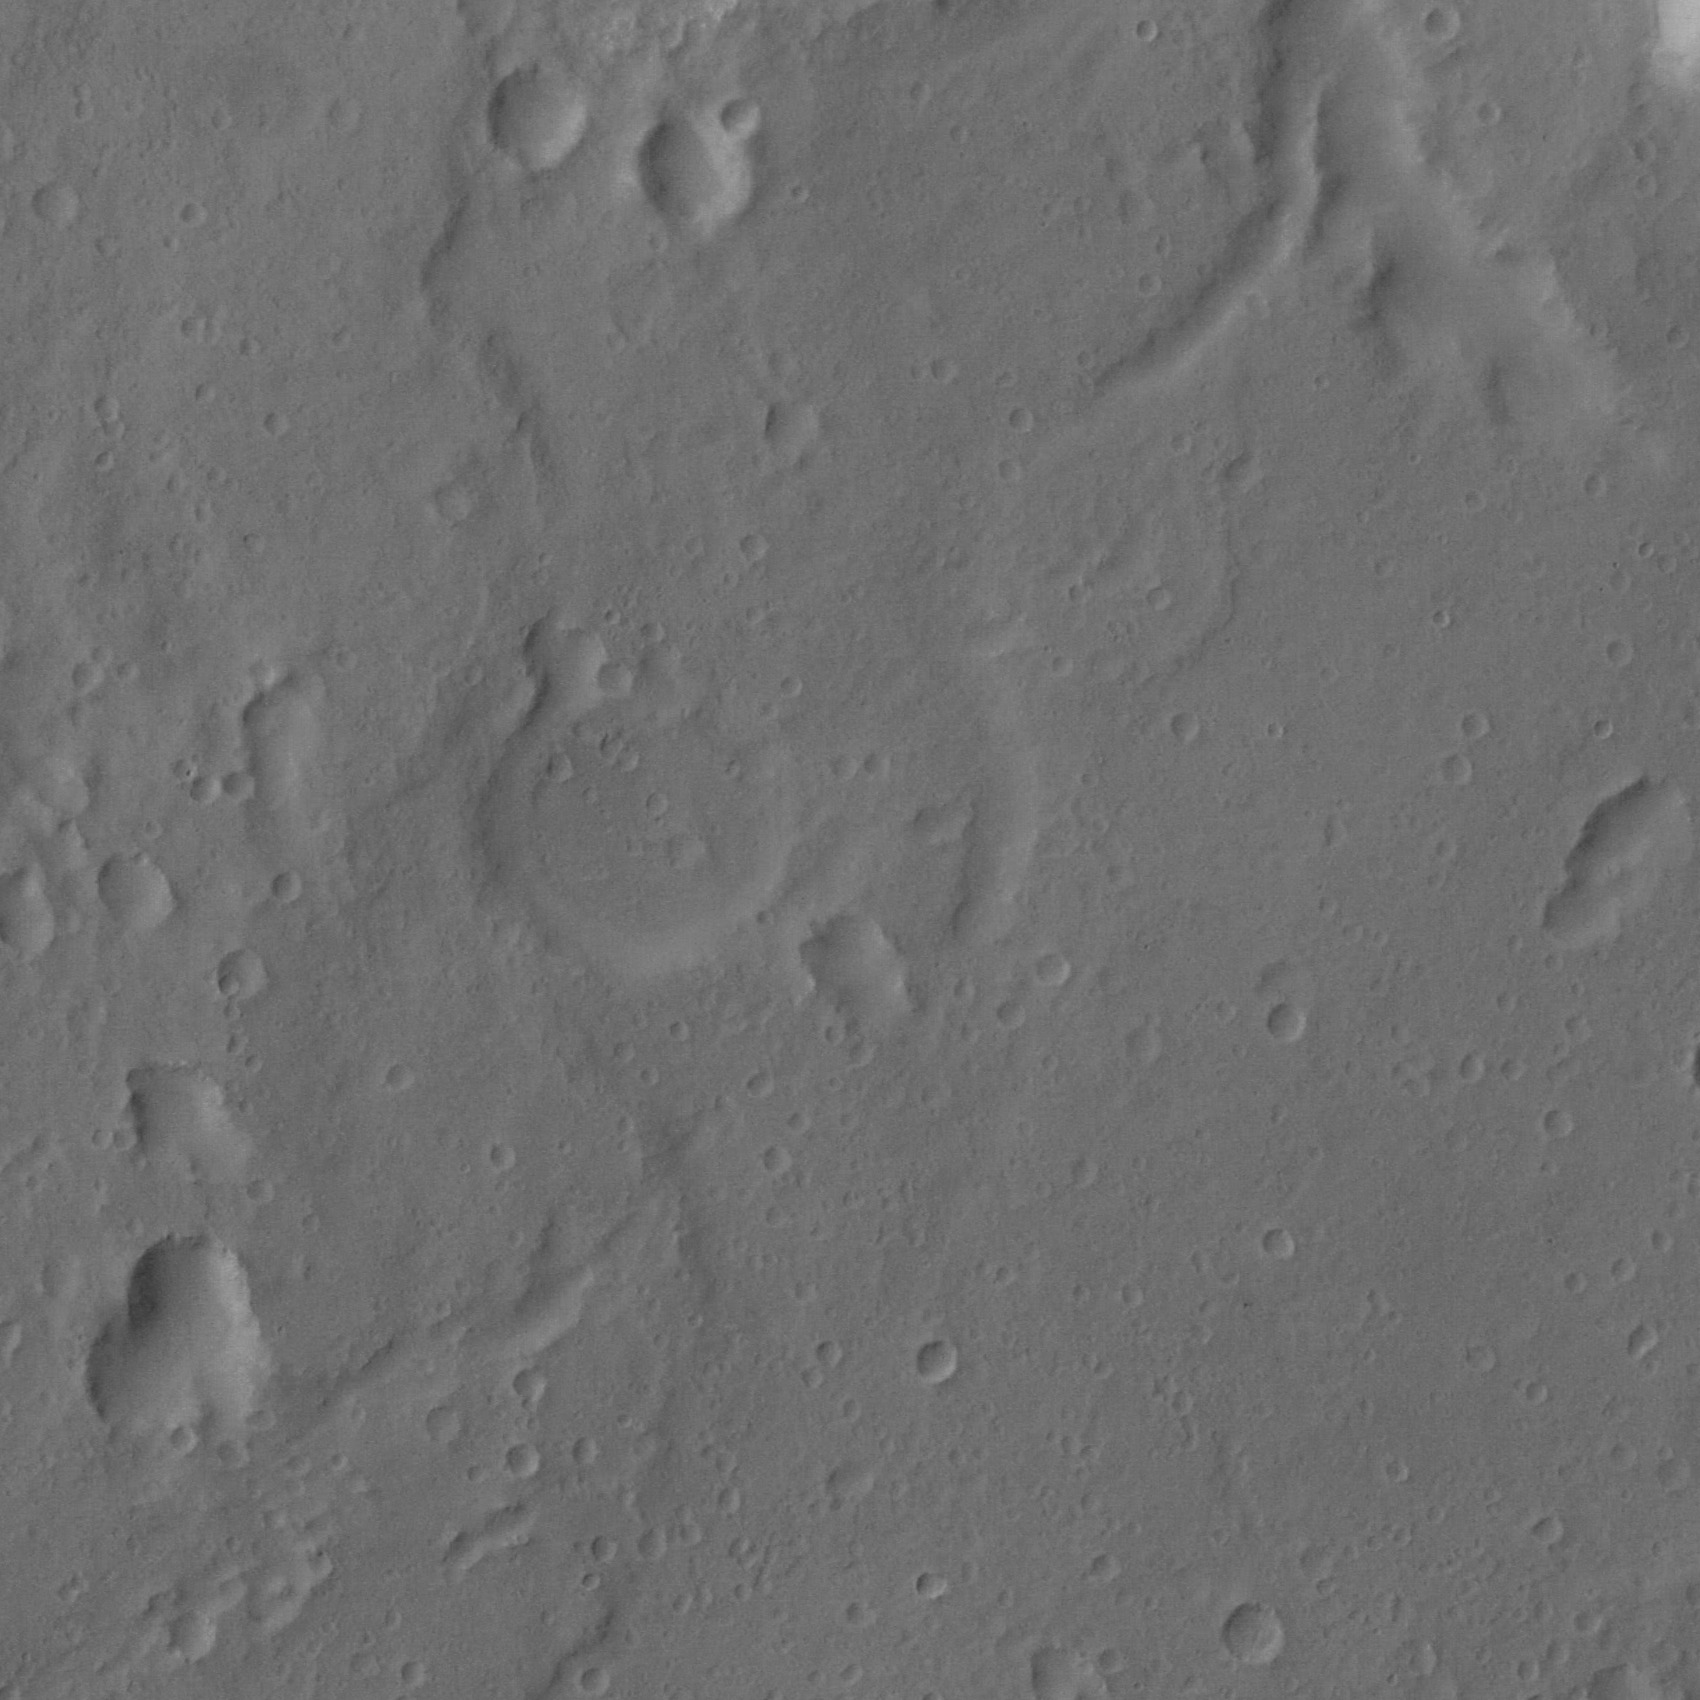
\includegraphics[width=\textwidth,keepaspectratio]{images/h0905_0000/1_24.jpg}
		\caption{1\_24}
	\end{subfigure}
	\begin{subfigure}{0.3\textwidth}
		\centering
		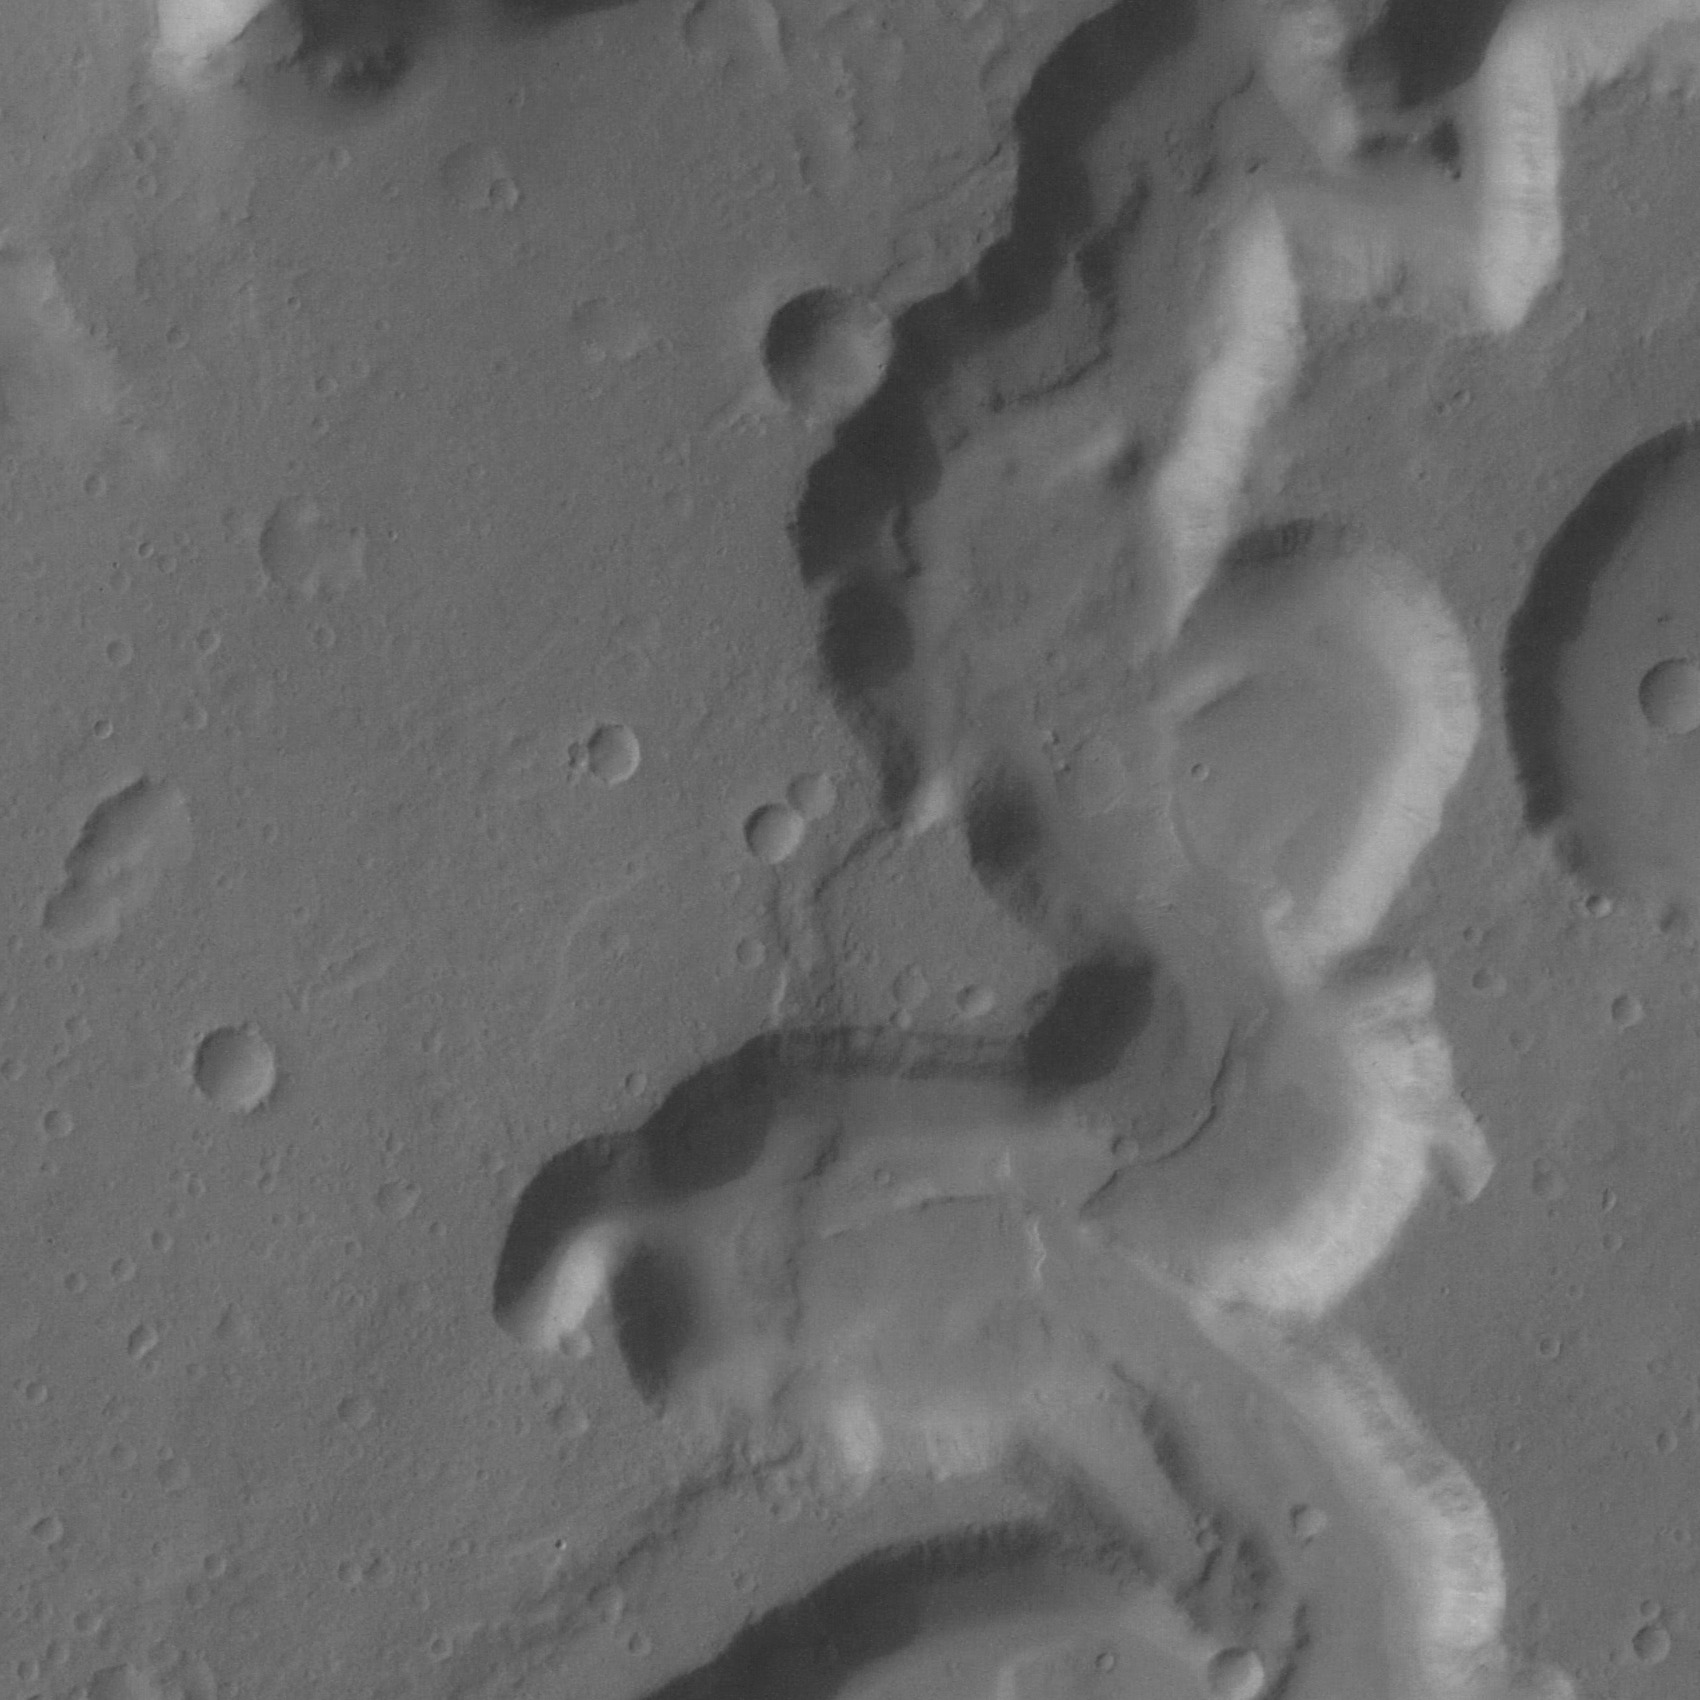
\includegraphics[width=\textwidth,keepaspectratio]{images/h0905_0000/2_24.jpg}
		\caption{2\_24}
	\end{subfigure}
	\begin{subfigure}{0.3\textwidth}
		\centering
		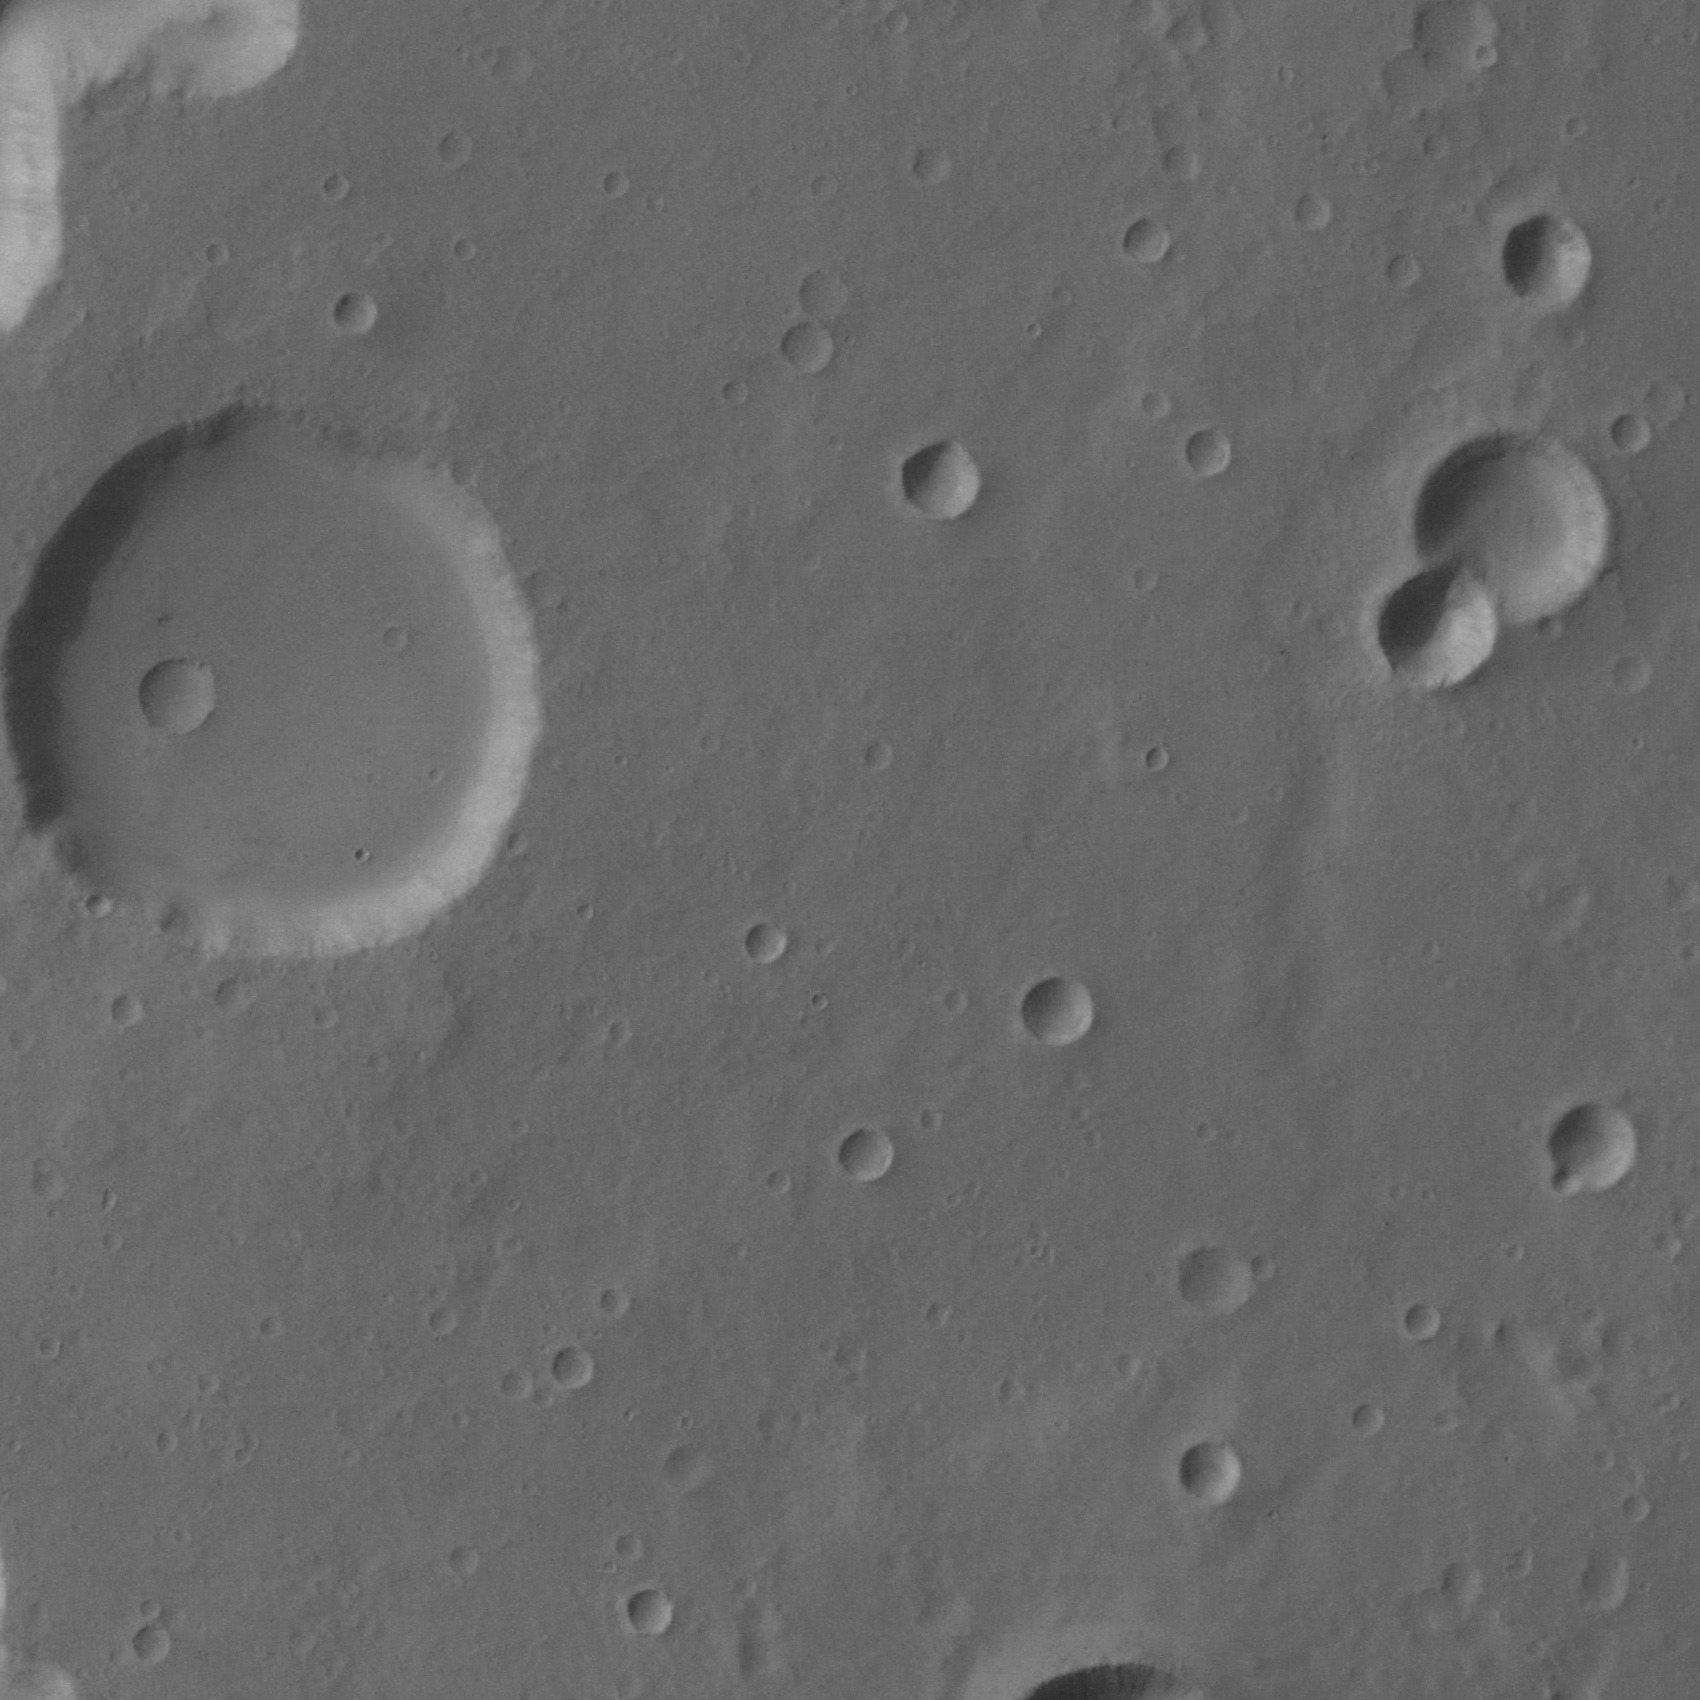
\includegraphics[width=\textwidth,keepaspectratio]{images/h0905_0000/3_24.jpg}
		\caption{3\_24}
	\end{subfigure}
	\begin{subfigure}{0.3\textwidth}
		\centering
		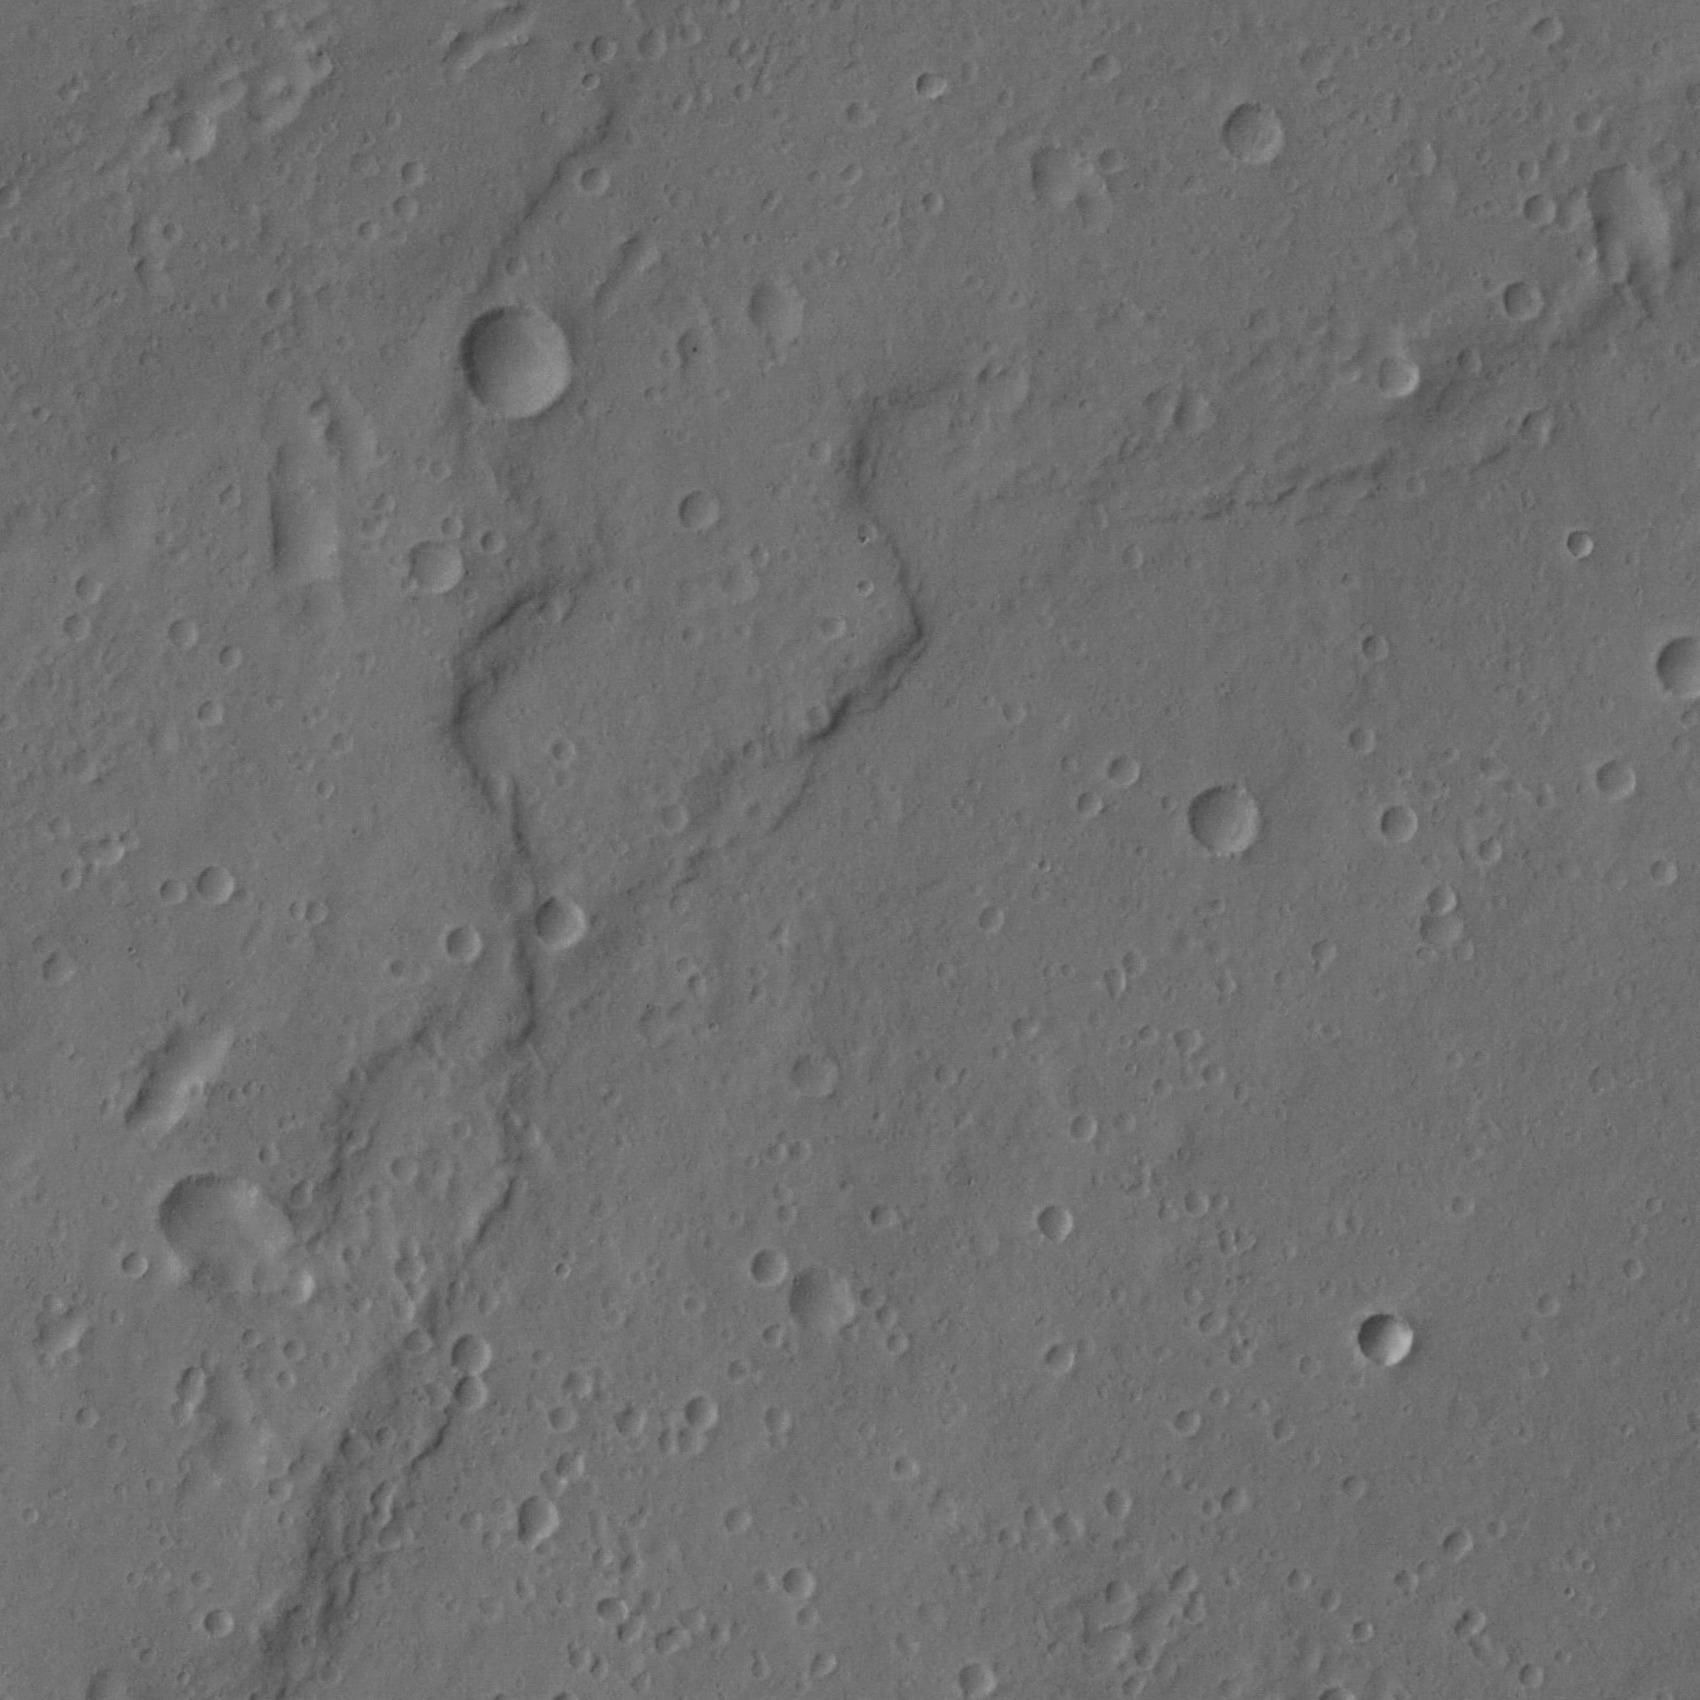
\includegraphics[width=\textwidth,keepaspectratio]{images/h0905_0000/1_25.jpg}
		\caption{1\_25}
	\end{subfigure}
	\begin{subfigure}{0.3\textwidth}
		\centering
		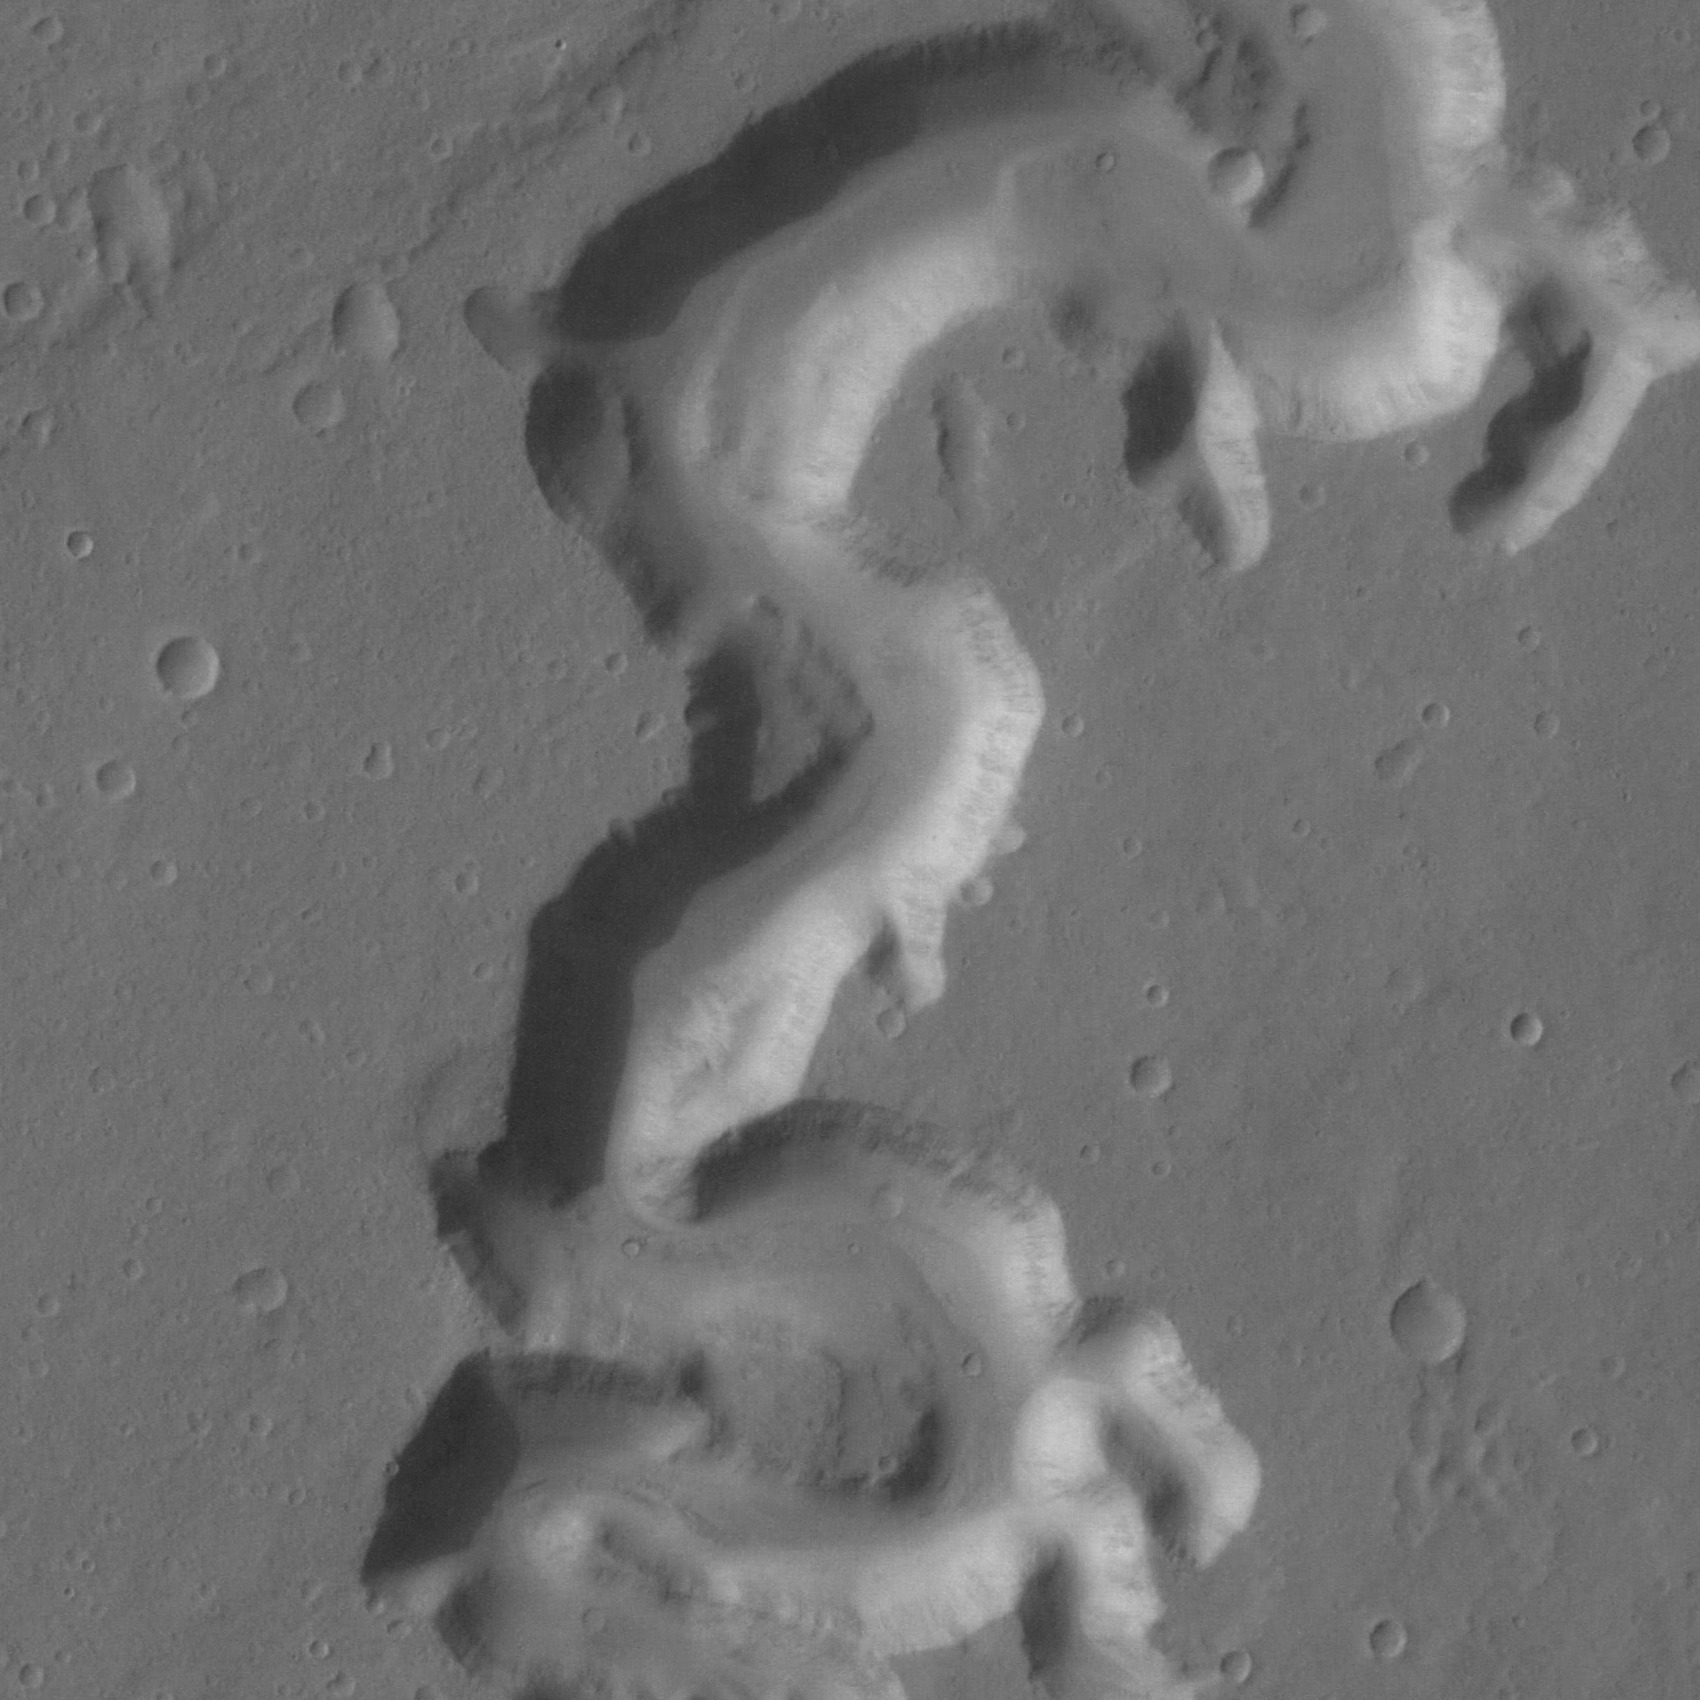
\includegraphics[width=\textwidth,keepaspectratio]{images/h0905_0000/2_25.jpg}
		\caption{2\_25}
	\end{subfigure}
	\begin{subfigure}{0.3\textwidth}
		\centering
		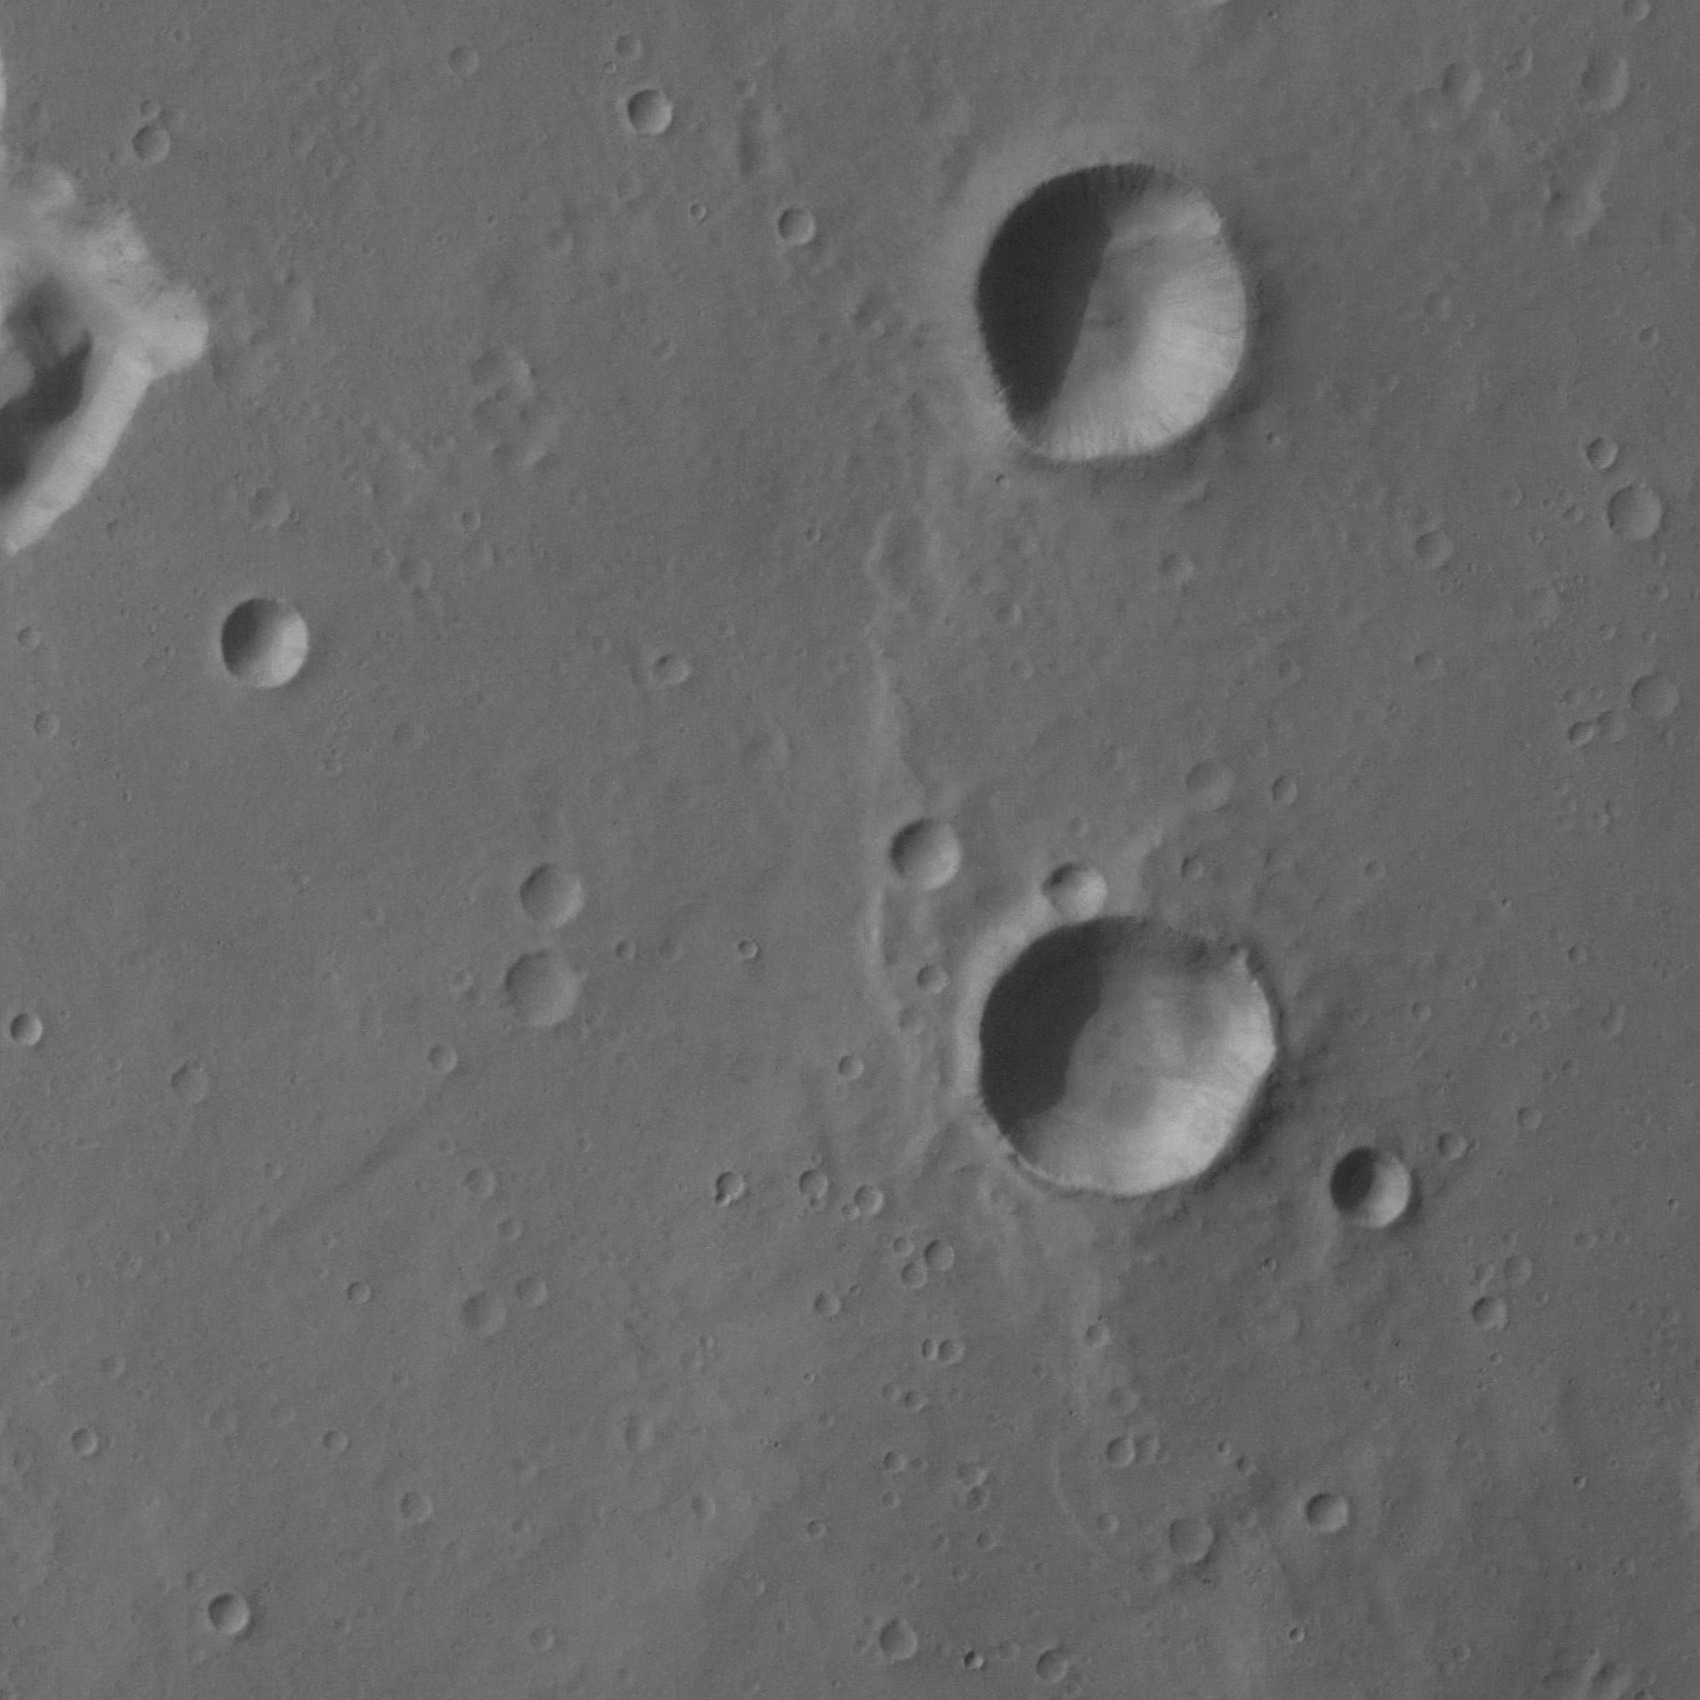
\includegraphics[width=\textwidth,keepaspectratio]{images/h0905_0000/3_25.jpg}
		\caption{3\_25}
	\end{subfigure}
	\caption{Die zur Evaluation genutzten Teilabschnitte}
	\label{fig:h0905_0000}
\end{figure}

\subsection{F1-Score zur Kratererkennung}
\label{ssec:f1_crater}

% TODO F1-Score definieren

In \tablename~\ref{tab:comparision} werden die in Abschnitt~\ref{sec:craterdetection} vorgestellten Methoden zur Kratererkennung verglichen.
Die F1-Scores für Urbach '09 und Bandeira '10 wurden aus den in \cite{bandeira_10} angegebenen \textit{True Positive}, \textit{False Positive} und \textit{False Negative} berechnet. Für Bandeira '12 konnte kein F1-Score berechnet werden, da dort die benötigten Werte nicht veröffentlicht wurden.

\begin{table}[h]
	\centering
	\begin{tabular}{l | s s s}
		Region & \text{Urbach '09} & \text{Bandeira '10} & \text{Cohen '16}\\
		\hline
		Westen & 67,95\% & 85,33\% & 88,78\% \\
		Mitte  & 69,63\% & 79,35\% & 88,81\% \\
		Osten  & 78,30\% & 86,09\% & 90,29\% \\
	\end{tabular}
	\caption{Die F1-Scores der vorgestellten Methoden}
	\label{tab:comparision}
\end{table}
\fi